


\documentclass[journal]{IEEEtran}
\usepackage[utf8]{inputenc}
\usepackage{graphicx}
\usepackage[sorting=none]{biblatex}
\addbibresource{bibliography.bib}

\begin{document}

\markboth{A survey of the danger that cyber terrorism poses in a cyber-centric world, December~2018}%
{A survey of the danger that cyber terrorism poses in a cyber-centric world, December~2018}

\title{A survey of the danger that cyber terrorism poses in a cyber-centric world, December~2018}
\author{Gary Connelly,~\IEEEmembership{Software Development (Honours),~GMIT}%
}


\maketitle

\begin{abstract}
Over the past couple of decades, cyberspace has opened the world up to a wealth of knowledge like it has never seen before. Today, anyone with a device that has the capabilities of connecting to the internet, has an absolute abundance of information right at their finger tips. The internet is possibly one of the most powerful tools man has ever created, helping nations, businesses and individuals operate much more efficiently. Does this efficiency come at a cost? This paper aims to review some of the articles and papers that take a thorough look into the possibility of humanities greatest tool being used as a weapon by various terrorist organizations. This paper will look at how the available literature defines and categorizes cyber-terrorism, the possibility of cyber-terrorism being adopted by terrorist groups, the possible effects cyber-terrorism could have on the world as well as some of the possible solutions that could be used to combat the threat of cyber terrorism.    

\end{abstract}

\section{Introduction}
Over the past number of years, the world has experienced an information explosion due to the rise of the internet. Information is now more available than it ever was before, making life infinitely more convenient and productive. However, this availability of information, and ease of connectivity between people has opened a door to malicious entities that could be very difficult to close. Cyber space allows much easier access to tools and information that could be used by terrorist organizations to further their agenda, recruit more members or to carry out more devastating and long term attacks than they have ever been able to execute in the past.

Most of the literature available on the topic of cyber-terrorism is quite new, some of the earliest papers that can be found are dated back to the early 2000s. One of the earliest relevant publications on the topic of cyber-terrorism \cite{verton2003black}, defines cyber-terrorism as "The execution of a suprise attack by a subnational terrorist group, or individuals with a domestic political agenda, using computer technology to cripple or disable a nation's electronic infrastructures." 
\bigskip 

This book also describes one of the first experiments ever carried out to investigate just how open the world, and America specifically are to a cyber terrorist attack. The experiment was was run by National Security Agency(NSA) and was code-named Eligible Receiver(1997). It goes on to describe how the experiment involved 35 NSA computer hackers that were told they could only use software tools and other hacking utilities that could be freely downloaded from the internet. The primary target for the 35 hackers, was the U.S Pacific Command in Hawaii, which is responsible for military contingencies and operations conducted in the Pacific theater. The results from this experiment were described as "chilling" \cite{adams2001virtual}. 

\bigskip

Posing as hackers from the North Korean intelligence service, the 35 hackers navigated their way through cyberspace mapping networks and logging passwords through various hacking methods such as brute force hacking and social engineering. The hackers were able to gain access to dozens of highly privileged Pentagon computer systems. With this level of access they would have been able to read and alter highly classified military documents and emails without ever being tracked. 

\bigskip

This experiment was possibly the first truly eye opening example of just how vulnerable America, and any other Nations that depend so much on the internet are to similar attacks. The number of publications of papers that looked into the subject of cyber-terrorism rapidly grew after the findings of this experiment.

\bigskip
This paper will systematically investigate some of the most relevant articles on the topic of cyber terrorism and attempt to answer questions such as "How imminent is the danger of cyber-terrorism is", "What are the consequences of cyber attacks on an international scale" and "How do we protect ourselves from such attacks". Section 2, Research methodology states the methods of research and research questions. Section 3, Classification is concerned with the different kinds of cyber-terrorism, section 4, Results looks into some of the solutions that could be implemented to help alleviate the danger as well as answering the research questions. Conclusions will be given in section 5, Conclusions.  

\section{Research methodology}
The steps I used to research for this paper were adapted from the Cruz-Benito paper \cite{cruz2016systematic} . His paper breaks the research down into five components; research questions, databases, search terms, inclusion/exclusion criteria, review phases.

\subsection{Research questions.}

The kind of questions that this paper will try to answer are as follows:

\textit{Question 1:} How does the literature define cyber-terrorism?\newline
\textit{Question 2:} Who is the most vulnerable to cyber-terrorist attacks?\newline
\textit{Question 3:} How do terrorist organizations use cyber space to further their agenda?\newline
\textit{Question 4:} What are the consequences to cyber-terrorist attacks?\newline
\textit{Question 5:} Is the threat of cyber-terrorism over hyped?\newline
\textit{Question 6:} What are the solutions to cyber-terrorism?\newline

Keeping these questions in mind will help greatly when studying the articles to review on this topic. 

\subsection{Databases.}

There were three main databases that were used when researching the literature for this review:\newline
\newline
- GMIT databases - (https://library.gmit.ie/databases/).\newline
- Google Scholar - (https://scholar.google.com).\newline
- IEEE Xplore - (https://ieeexplore.ieee.org).\newline

\subsection{Search terms.}
For starters, the phrase "cyber-terrorism" was the key search term used in these databases. This, however yielded a result set that was way too big to go through so it was important to start doing more advanced searches to find the more relevant publications. The search was later confined to publications that had that phrase in the title, along with review, survey, vulnerabilities, solutions, threat, financial and national in the title of the article. The abstract of each article would then be investigated to determine its suitability for this paper. The more suitable papers that were found would then be categorized into three sections; vulnerabilities, consequences and solutions.
\bigskip

By doing this, I was able to get the initial result set down from over 17,000 results, to less than 100.
\newline
\newline

\includegraphics[width=250]{1stSearch.PNG}
\newline
\newline
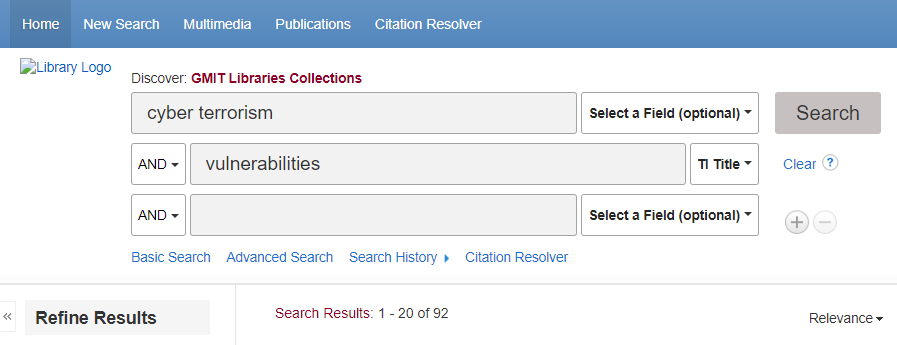
\includegraphics[width=250]{2ndSearch.PNG}


\subsection{Inclusion and Exclusion criteria.}
In order to have more efficient research take place, there had to be some immediate inclusion and exclusion drafted out do determine straight away whether an article should even be investigated or not. The inclusion criteria included; the article must be peer reviewed, full text must be available, must be in English. \newline Some of the exclusion criteria included; studies that are not related to the search terms, publications where the full text was not publicly available, publications that are not in English.

\subsection{Review phases.}
The review phase took the form of the following steps:\newline
\newline
- First the articles are searched in the three databases mentioned above.\newline
- The result set is narrowed down via the exclusion criteria.\newline
- The result set is further narrowed down by reading the full abstract and possibly the introduction, and removing the irrelevant articles.\newline
- Result set is further narrowed down by reading the different topics discussed in the remaining articles, and again removing irrelevant articles.\newline
- Out of the remaining articles, study them in their entirety.\newline

The remaining articles and publications from this exercise would be the literature to review for this document. 

\section{Classification of the literature.}
After the research of the topic was executed following the steps outlined in the research methodology, about 20-22 publications were thoroughly studied. Out of all of the publications that were studied, most of them appeared to discuss the topic in one or more of the four following categories; defining cyber-terrorism, how terrorist organizations use cyber space, the economic consequences of a cyber-terrorist attack, and the national/international consequences of a cyber-terrorist attack.

\subsection{Defining cyber-terrorism.}
As the study of the remaining articles continued, it was becoming increasingly noticeable that most of the publications had similar, but ultimately differing opinions on how cyber-terrorism should be defined.\newline
Vida  M  VILI � C  \cite{vilic2017dark}   describes cyber-terrorism as "Cyberterrorism, as a part of the cyber warfare, refers to deliberate, politically motivated attacks on computer systems and
programs, as well as spreading the data which could provoke violence and
fear with the civilian targets, in order to persuade the government to change
its policy ".\newline Vida  M  VILI � also suggests cyber-terrorism and cyber warefare have the same characteristics. Michael  L  Gross, Daphna Canetti, and Dana R Vashd \cite{gross2016psychological} discuss the differences between cyber-terrorists and cyber-criminals, suggesting while the lines are blurred between the two entities, it is typically the motivation of the assailant/s that determines whether or not they are committing an act of terrorism or criminalism. The paper goes on to say that criminals are motivated by financial gain, "criminals out for pecuniary gain", where as terrorists are typically politically motivated, "But sometimes their motives are political."\newline
In a 2015 paper, Michael   Kenney \cite{kenney2015cyber} described cyber-terrorism as "computer to computer voilence".

\subsection{How terrorist organizations use cyber-space.}

Throughout the study of these publications, it became clear that there are different ways in which terrorist organizations use cyber-space depending on what their immediate goal was. Vida  M  VILI � \cite{vilic2017dark} and F Saidi, \cite{saidi2017approaches}  describe some of these methods. They explain how cyber space is the perfect place for glorifying terrorist attacks because of the fact that is it so easy to spread news all around the globe. Through this use of propaganda, the terrorist organizations can then move towards using cyber-space to recruit more members to their cause. This is made possible due to the fact that cyber-space is not limited to any physical location. "it is a "space" bounded only by screens and passwords rather than physical markers", David R Johnson  \cite{johnson1996law} states in his 1996 �Law  and  borders:The rise of law in cyberspace". This allows for a much cheaper, and more rapid spread of extremist ideologies. These organizations also came up with very clever ways of communicating through cyber-space.\newline Dorothy  E  Denning \cite{denning2010terror}, describes how terrorists used a method called a "dead drop" to communicate with each other. This involves multiple members of an organization having one email account between them. Whenever they wanted to communicate with each other, they would simply write their message and save the email in the "drafts" folder. When the other members would log into this account, they would simply look in the drafts folder to see the message. This way, there were no messages being transported over networks making them impossible to intercept and decrypt. \newline

This summarizes what the literature suggests that terrorist organizations do with cyber-space and how cyber-space helps them operate, without actually going into how these organizations use cyber-space to actually carry out attacks. The next two parts of this classification will review that part of the literature in more detail. 

\subsection{Economic consequences of cyber-terrorism.}
"Modern economies are heavily dependent upon Information Technology (IT) based information systems for survival. Increased reliance on information systems (ISs) leads to increased vulnerabilities and risks. IS security has thus become a critical issue in the IT world" \cite{hua2013economic}. Jian Hua and Sanjay Bapna's journal titled �The economic impact of cyber-terrorism� talks about how a single cyber-terrorist attack on on key financial institutions , "such as the national/federal banks", could result in an over all destabilization of national and even international economies.
Patrick Lenain, Marcos Bonturi, and Vincent Koen\cite{lenain2002economic}, discuss how terrorism in general can cause long term macro-economic affects on the economy, making the example of how the September 11th attacks had huge knock on affects from an economic perspective. They go on to talk about "shrinking insurance coverage stemming from the perception of greater risk, higher trade costs possibly affecting international trade, and stepped-up security spending partially rolling back the �peace dividend� of the 1990s." These publications make the argument that any attack on a major financial system can have huge adverse affects for not only the economy of the target to the attack, but the world economy as a whole. 

\subsection{National/International consequences of cyber-terrorism.}
The literature on this topic seems to suggest that the national/international consequences of cyber terrorism, and the economic consequences are not mutually exclusive. For example, Michael Kenny \cite{kenney2015cyber} describes the infamous 2010 stuxnet attack on the Iranian nuclear plant. This virus was able to infect the  computers operating the centrifuges, causing the destruction of over half of the centrifuges over a space of a month. This attack was said to set Irans nuclear operations back about 2 years and billions of dollars. This is possibly the most famous example just how damaging a well executed cyber attack can be. \newline
Julia  E  Sullivan  and  Dmitriy  Kamensky \cite{sullivan2017cyber}, explain how cyber attacks against the Ukrainian power grid expose vulnerabilities across the globe. They describe how on December 23th 2015, a cyber-attack caused six hour black outs for hundreds of thousands of people in the city of Kiev. They make the case that the same sort of attacks can just as easily be executed against any other country that is on the grid "the attack methodology, tactics, techniques and procedures that were successfully deployed in Ukraine could be deployed against infrastructure here and around the world".  \newline Robin Gandhi \cite{gandhi2011dimensions} talks about how essential systems, such as those providing water, finance, food, health care electricity and transportation are becoming increasingly software dependant and interconnected. This exposes any of these systems to the possibilities of being attacked by organizations of hackers or terrorist groups. 

\section{Results}
This section of the literature review is responsible for answering the questions posed in the research methodology section.

\textit{Question 1:} How does the literature define cyber-terrorism?\newline
\newline
To find an answer to this question, adding the search terms "survey", "explained", and "definition" was necessary. As mentioned earlier in this literature review, there seems to be multiple similar but different meanings for the term "cyber-terrorism". The literature studied for this review seems so be concurrent on the fact that it is the use of the internet/cyber-space to carry out politically motivated attacks or to spread an ideological doctrine.  \cite{vilic2017dark},           \cite{gross2016psychological}, \cite{kenney2015cyber} .
\newline
\textit{Question 2:} Who is the most vulnerable to cyber-terrorist attacks?\newline

Over the past century, war fare has mainly been concentrated in the middle eastern, sometimes third world countries. However, cyber-warfare flips this premise on it's head. \cite{lewis2002assessing} James Andrew Lewis talks about "critical infrastructure" being the main target for cyber attacks, meaning that wealthy developed countries are the most vulnerable to these types of attacks. This danger is then compounded by the fact that it is relatively cheap for organizations to carry out cyber attacks in comparison to more traditional war tactics \cite{vilic2017dark}. 
\clearpage
\textit{Question 3:} How do terrorist organizations use cyber space to further their agenda?\newline
\newline
The articles that were studied in order to complete this review highlighted some of the main ways terrorist organizations use cyber space to function.  \cite{vilic2017dark} Vida M VILI �'s publication was one of the more explanatory documents discussing how these organizations use cyber space. The main uses being; glorification of terrorist attacks, recruitment, communication, and carrying out devastating attacks on a cheaper, safer budget.\newline

\textit{Question 4:} What are the consequences to cyber-terrorist attacks?\newline
The literature on this topic suggests that there are two main consequences of cyber-terrorism, being economic consequences, and national/international consequences, which have been discussed already, with a possible third kind of consequence being psychological. \cite{gross2016psychological} Michael L Gross, Daphna Canetti, and Dana R Vashd and their paper "The psychological effects of cyber terrorism" was the only piece of literature studied for this survey that went into detail on some of the possible psychological impacts cyber-terrorism could have on the victims. Their paper also states there is a clear connection between the perception of threat of cyber terrorism and militant hardline attitudes. They go on to say that people would be more willing to "support surveillance, government regulation, and military retaliation compared to those whose threat perception is lower."\newline

\textit{Question 5:} Is the threat of cyber-terrorism over hyped?\newline

While most of the publications that were studied for this review were concurrent in agreeing that cyber-terrorism is a very real threat, some publications seemed to disagree on just how immediate the danger is. Richard A Clarke \cite{clarke2016risk}, for example stated that while a full scale cyber war will happen at some stage in the future "it most certainly will", however that the mere fact that this technology exists does not in and of itself increase the likely hood of a war. He goes on to state that "governments will only engage in "total" cyber war within the context of a war that they were already going to fight militarily otherwise." However, it would appear that some publications seem to disagree with this, stating, for example that the stuxnet attack could only have been engineered by a government state, making it an act of cyber war that has already taken place \cite{kenney2015cyber}. This was the only research question that was difficult to answer given the available literature.\newline

\textit{Question 6:} What are the solutions to cyber-terrorism?\newline

Because of the fact that cyber-terrorism is a relatively new concept, it proved rather difficult to find literature that would provide concrete answers to this research question.However, Keman  Huang, Michael  Siegel,  and  Madnick  Stuart \cite{huang2018systematically} believe that the key to alleviating the danger of cyber terrorism, is understanding the cyber attack business. Their paper provided a really interesting take on how this issue could be tackled. They propose a "value-chain" model that is designed to better understand the motives of the attackers and the process that attackers go through in order to carry out an attack. They suggest that if we can understand the motives and processes that attackers use, we would be more equipped for coming up with a deterrent. 

\subsection{Conclusion.}
With each passing day, we become more and more dependant on the internet and all the critical infrastructure that is connected to it. The more dependant we become on critical technology, the more we open ourselves up to potentially devastating attacks from the various terrorist organizations that might want to target the critical infrastructure. \newline
The body of literature surrounding this topic has been growing at a steady rate since the late 1990s, but has exploded in the years following the 2010 stuxnet attack. Out of the literature that was reviewed in this case, most of it was concerned with understanding the problem and trying to figure out how imminent the danger is. The available literature regarding what the problem is, the ways in which cyber space can be used as a weapon, and where the vulnerabilities are, was very extensive and well informed. However, there was an alarming lack of reliable literature available that was looking into how to solve potential future threats of cyber-terrorism. It is also entirely possible that the literature concerning solutions to the problem does exist, but for one reason or another e.g. the exclusion criteria, I just didn't happen to come across much of it.

\section{Bibliography}

\printbibliography
\end{document}


